\documentclass[tikz,border=10pt]{standalone}
\usepackage{amsmath}
\usetikzlibrary{angles,quotes}
\begin{document}
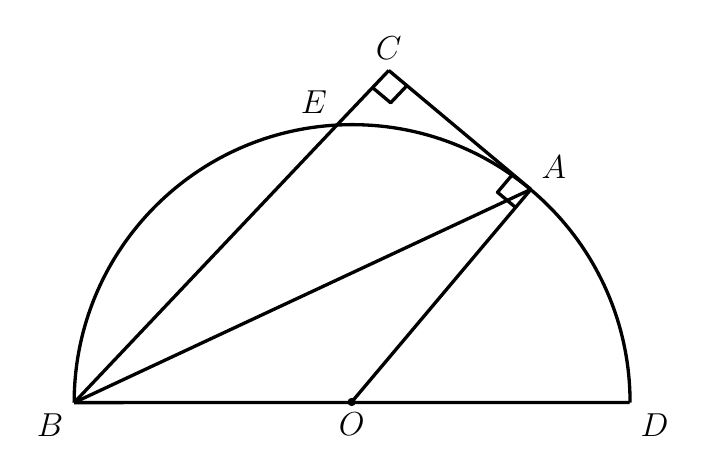
\begin{tikzpicture}[line join=round, line width=1.2pt]
\coordinate (A) at (2.251,0.605);
\coordinate (B) at (-3.549,-2.103);
\coordinate (C) at (0.447,2.115);
\coordinate (D) at (3.506,-2.101);
\coordinate (O) at (-0.024,-2.095);




\coordinate (E) at (-0.202,1.432);


\draw (B) arc[start angle=180.000, delta angle=-180, radius=3.530];


\draw (B) -- (D);
\draw (B) -- (E) -- (C);
\draw (C) -- (A);
\draw (A) -- (B);
\draw (A) -- (O);


\fill (O) circle (1.500pt);


\pic[draw, angle radius=0.300cm, angle eccentricity=1.25] {right angle=B--C--A};
\pic[draw, angle radius=0.300cm, angle eccentricity=1.25] {right angle=C--A--O};


\node[above, font=\fontsize{12.5}{15}\selectfont] at (C) {$C$};
\node[above left, font=\fontsize{12.5}{15}\selectfont] at (E) {$E$};
\node[above right, font=\fontsize{12.5}{15}\selectfont] at (A) {$A$};
\node[below left, font=\fontsize{12.5}{15}\selectfont] at (B) {$B$};
\node[below right, font=\fontsize{12.5}{15}\selectfont] at (D) {$D$};
\node[below, font=\fontsize{12.5}{15}\selectfont] at (O) {$O$};
\end{tikzpicture}
\end{document}